\section{Video Similarity Application}
To perform computations on encrypted floating-point numbers, we utilize the CKKS scheme [11] with a polynomial modulus degree of 4096. CKKS is a homomorphic encryption scheme to perform computations of approximate arithmetic on real numbers. This scheme offers out-of-the-box support for decimal value computations compared to other schemes like BFV and BGV, which primarily focus on integer arithmetic. The choice of 4096 as the polynomial modulus degree balances the need for strong security and accuracy with practical computational performance. While a larger degree enhances security and allows for more operations before result degradation, with the trade off of increasing computation time and ciphertext size.

In order to detect similarities between the two videos, we represent each video as a probability distribution of byte size changes between one-second segments, shown in Figure \ref{fig:preprocess-data-flow}. To transform raw video into comparable probability distributions, we count the number of bytes in each frame, calculate the sum of frame lengths in each segment, and then normalize the array of segments between zero and one, known as a Probability Distribution Form (PDF), ensuring that the distributions for both videos have the same scale and can be directly compared. This re-implementation of Proof of Presence Share \cite{Lagesse2021-PopShare} provides strong privacy guarantees, as if the encryption is broken, the raw byte data cannot be reconstructed from the normalized byte array due to the loss of information during the aggregation and normalization process. Alternative approaches include a motion estimation approach with the Lucas-Kanade method \cite{Lucas1981-uy} supported by OpenCV, which could provide more detailed information about video content. However, for this study, it is crucial to compare our approach to the established baseline metrics, and new methods would hinder this comparison.

\begin{figure}[t]
    \centering
    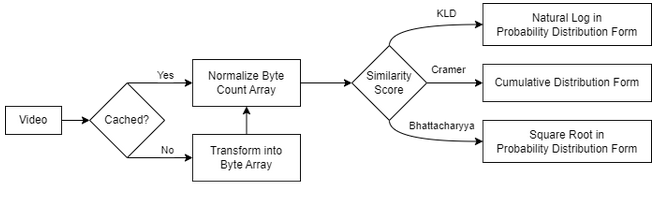
\includegraphics[width=\textwidth]{4 Design/4.3 Preprocess Data Flow.png}
    \caption{Pre-process Data Flow}
    \label{fig:preprocess-data-flow}
\end{figure}

To compute multiple similarity scores using homomorphic encryption, separate byte arrays are encrypted for each score. The recipient can perform computations with plaintext decimal values against the corresponding encrypted element in the array. This approach leverages the unique ability of fully homomorphic encryption and was borrowed from Pop-Share, as this approach is much faster than comparing ciphertext against ciphertext. 

For Kullback-Leibler Divergence, we share the PDF and its natural log. For each encrypted double in the PDF, we subtract the natural log of the plaintext element and multiply the difference. The product remains encrypted and is returned to the originator, where it can be decrypted. The summation is the similarity score.

For Bhattacharyya Coefficient, we share the square root of the PDF. For each encrypted double, we multiply the ciphertext by the square root of the plaintext element. The product remains encrypted and is returned to the originator, where it can be decrypted. The summation is the similarity score.

For Cramer Distance, we share the Cumulative Distribution Form (CDF) from PDF. The CDF is the cumulative sum of all of the elements in the PDF, such that the last value of CDF is equal to 1. For each encrypted double, we square the difference of the plaintext element. The product remains encrypted and returned to the originator, where it can be decrypted, and the square root of the summation is the similarity score.

In order to share the encrypted byte-count arrays, GhostPeerShare packages all ciphertext objects into an archive. The encrypted parameters and any associated data are stored as binary files, with each algorithm (e.g., $kld\_logX$) using 60 binary files, each representing one second of a one-minute video. This structure is particularly helpful for cases where video lengths differ, as it simplifies the trimming process. The binary files are then archived into an \textit{.enc} file format, which is unique to our application and contains both the encrypted data and a metadata JSON file with relevant video details (e.g., timestamp, length, frames per second). The archive averages around 40 MB on Linux for 1 minute of video.

\begin{figure}[t]
    \centering
    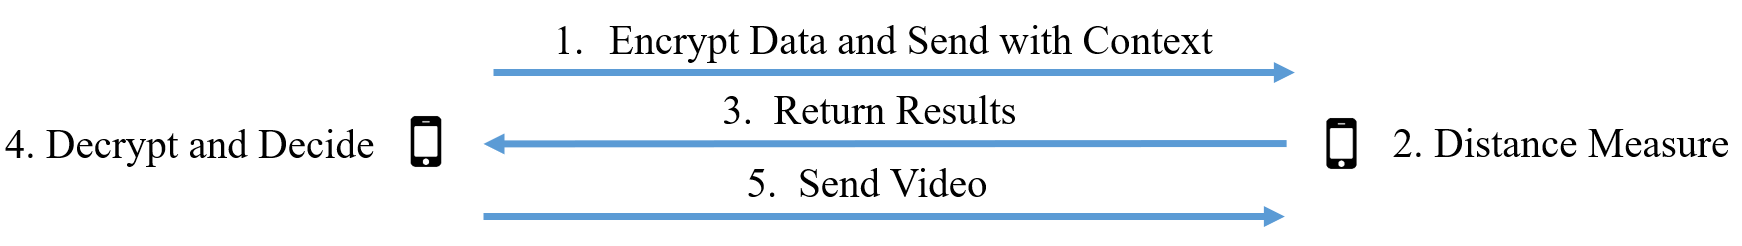
\includegraphics[width=\textwidth]{4 Design/4.3 Peer-to-Peer.png}
    \caption{Peer-to-peer Data Flow}
    \label{fig:peer-to-peer-data-flow}
\end{figure}

To facilitate a peer-to-peer exchange of files shown in Figure \ref{fig:peer-to-peer-data-flow}, GhostPeerShare supports QuickShare \cite{samsung_quick_2020} for Android devices. QuickShare [10] was developed by Samsung as a file-sharing utility application for nearby wireless devices. It leverages Bluetooth to discover nearby wireless devices and optionally uses WiFi to transfer large files between two nodes. QuickShare is accessible through a Flutter plugin that enables users to share data using their device’s native sharing capabilities. This allows each node to asynchronously send and receive files, leveraging a built-in Android feature rather than embedding similar functionality within the Flutter application.
